\chapter{Analysis}

To begin, Sarmento et al.'s \cite{Sarmento2014} review paper is a great representation of the existing research in the field, along with the difficulties surrounding their eligibility and applicability to exploring the question at hand. 

Starting off with 2732 titles (sourced in 2014) from the Institute for Scientific Information database, they were filtered using the keywords football and soccer, each one associated with the terms: match analysis, performance analysis, notational analysis, game analysis, tactical analysis and patterns of play. This filtering process resulted in only 53 articles being chosen for incorporation into the review based on eligibility, demonstrating the capability for more research to be conducted in the field. Papers were then filtered further into categories dependent on the type of analysis that was conducted. 

\subsection{Descriptive Variables}
First, descriptive variables- described as variables that are related to what takes place during a match- were analyzed, specifically in relation to player activity. One study, conducted by De Baranda et al. \cite{DeBaranda2008} targeted goalkeepers and examined how their movements vary throughout a match. It was found that goalkeepers covered a total distance of $5611 \pm 613$ m per match, of which $221 \pm 90$ m was spent running, $56 \pm 34$ at high intensity running, and $11 \pm 12$ sprinting. 

Soccer can be described as a non-cyclical sport that primarily incorporates a combination of short-duration maximum-intensity activities, light to moderate jogging, and pauses. A study, conducted by Andrzejewski et al. \cite{Andrzejewski2013}, describes the sprinting activities of professional soccer players during Europe League matches in the 2008 - 09 and 2010 - 11 seasons. Two types of sprints were distinguished based on their duration: S, short-duration sprint (below 5 seconds) and L, long-duration sprint (above 5 seconds). Additionally, sprints were classified according to their distance: 0–10, 10.1–20.0, and .20 m, respectively. The players were also analyzed with taking their positions of play into consideration. 

The results \cite{Andrzejewski2013} reveal that players, on average, covered a total sprint distance of $237 \pm 123$ meters, with forwards covering the longest distances ($345 \pm 129$ meters), suggesting a position-specific demand for sprinting activities. The average number of sprints performed by the players was $11.2 \pm 5.3$, and players perform 2- to 4-second long-sprint runs on average, which translates to only about 1- 3\% of match time spent actually sprinting. Regardless, they tend to sprint long distances, with the average sprinting distance covered during a match being between 200 and 1,200 m across all positions, a significant difference from the time spent sprinting by goalkeepers. 


\subsubsection{Methods} 
147 players, excluding goalkeepers, participating in 10 matches across the league were first assigned to one of 5 position groups (central defenders (CD), external defenders (ED), central midfield (CM), external midfield (EM), and forwards (F). Using the Amisco Pro tracking system, their sprinting activity was analyzed. Descriptive statistics were calculated for the parameters, calculating means, medians, IQR, etc. 

Multifactor ANOVA was then utlized to determine if means across groups of positions were significantly different, and  values were analyzed at a 95\% confidence level. If ANOVA indicates a significant difference, post-hoc tests like Tukey's was used to identify where exactly the differences lie. For example, if ANOVA shows that total sprint distance was statistically different across positional groups, the Tukey test identifies specifically that forwards sprint significantly more than midfielders and defenders.
\newline
\begin{table}[ht]
\centering
\begin{tabular}{p{0.3\textwidth}p{0.3\textwidth}p{0.3\textwidth}}
\hline
Activity & \multicolumn{2}{c}{Identified Results} \\
\hline
Total sprints & \multicolumn{2}{p{0.6\textwidth}}{Forwards (F) performed more total sprints than Central Midfielders (CM) and Central Defenders (CD). External Midfielders (EM) also performed more total sprints than CD and CM.} \\
Short-duration sprints & \multicolumn{2}{p{0.6\textwidth}}{Forwards (F) and External Midfielders (EM) performed more short-duration sprints than Central Defenders (CD) and Central Midfielders (CM).} \\
Long-duration sprints & \multicolumn{2}{p{0.6\textwidth}}{External Defenders (ED) performed more long-duration sprints than Central Midfielders (CM).} \\
\hline
\end{tabular}
\caption{Statistically Significant Differences in Sprinting Activities Among Different Player Positions.}
\label{tab:sprinting_activities}
\end{table}
\newline
Another study, conducted by Jamil et al., \cite{Jamil2021} analyzed the performance of teams in England, Germany, and France’s second divisions over 5 seasons in order to gain an understanding of factors that influence the football teams' promotion chances from second-tier leagues to elite leagues in Europe. Analyzing a vast dataset of 11,032 team-match observations over five seasons, the study employs logistic regression to evaluate the impact of various performance indicators on the likelihood of promotion.

This research splits technical indicators into defensive metrics, set-piece execution, and passing strategies, assessing their predictive power for promotion success. Notably, the study highlights that a team's defensive workload, evidenced by actions such as blocks, clearances, and goalkeeper saves, negatively correlates with promotion chances. Conversely, it identifies set-pieces, particularly penalty kicks and corner kicks, as significantly positive for promotion prospects, with successful penalties and goals from corners increasing promotion odds by 37\% and 35\%, respectively. Assists are also major contributors to promotion likelihood, increasing odds by 24.6\%. \cite{Jamil2021}



\subsection{Comparative Variables}
Sarmento et Al. then proceeded to identify their next categorical variable as comparative variables, specifically variables that compare different situations and gauge how parameters varied across these situations. The previous study conducted by Andrzejewski et al. was a great example of comparative variables in use as well, as the relationship between the player’s positional role and performance was examined. This is a very common parameter that is explored due to its efficacy in preparing players for game day. A pivotal study by Rampinini et al. \cite{Rampinini2009} provides an insightful perspective by comparing the technical and physical performances of players from the Italian Serie A league, highlighting the influence of fatigue and competitive level on match performance, across two established levels: successful teams (ranked in the
first five positions) vs. less successful teams (ranked in the last five positions).
This study was the first to examine the relationships between physical performance during the match and team success amongst a homogenous group of professional soccer players competing within the same national league

\subsubsection{Methods} 
Using unpaired t-tests, Rampini at. al were able to discern significant differences in physical and technical performance between more and less successful teams. In order to counteract the problem of multiple comparisons, Bonferroni's correction was used to tighten the criteria for statistical significance and assigned an alpha value of 0.01. At this adjusted significance level, involvements with the ball, short passes, successful short passes, tackles, dribbling, shots and shots
on target were higher in the more successful group than in the less successful group. Other physical and technical factors did not prove to have any significant differences across successful and unsuccessful teams. 
Interestingly enough, another study conducted by Mohr et al. also looked into the effect of fatigue over the course of a match, as well as total distance, high intensity running, and sprinting distance of players in Italy's Serie A league and compared them to the activities of players in the Danish professional League \cite{Mohr2003}. Rampini et al.'s \cite{Rampinini2009} study shows us that players from successful teams tend to cover less distances at all speed ranges compared to their less successful counterparts, but they tend to do more physical work when in possession of the ball. Mohr et al.'s study, however, indicates that players in Serie A consistently performed more high-intensity activity than lower level professional players participating in the Danish League. This provides an interesting distinction that although top-level players in Serie A engaged in more high-intensity play overall, being part of a successful team as noted by Rampini et al. seems to correlate more with effective work—particularly with the ball—rather than merely increased physical activity across the board. This identifies league context and a team's tactical approach to be influential in match success, but also provides the base for further research in the space that answers questions such as: whether these findings are consistent across other leagues, or how teams can leverage these insights for inter-league match preparation. 

A study conducted by Bradley at al. \cite{Bradley2010} also pinpoints high-intensity running as it's paramter of chocice. Unlike Andrzejewski et al,'s \cite{Andrzejewski2013} focus which was on analyzing sprinting activities across positions, this study aimed to delineate the high-intensity activity patterns of soccer players at different performance levels (elite domestic vs. elite international) and playing positions. The levels were established as Elite domestic players (that played in teams that compete in one of the strongest leagues in the world) vs. Elite international players (that played in teams ranked in the Top 10 of the FIFA rankings). The results of this study were unexpected as well, as there were no significant differences found in high-intensity running distances between elite domestic and international players, suggesting uniformity in physical demands at the top levels. However, similar to the non-comparative study, positional analysis revealed that wide midfielders and forwards performed more high-intensity running than defenders. It's important to note that the study does not explicitly discuss how the potential overlap in players and play styles can be accounted for, as the top domestic leagues across the globe also tend to be composed of the players that rule the international level, so the homogeneity in high-intensity running performances might reflect a universal standard of physical conditioning and tactical implementation among elite soccer athletes. 


\subsubsection{Data Normalization}
An important methodology in the context of analyzing comparative variables is data normalization, first introduced by Hughes and Franks \cite{Hughes2005}. In their study, they sought to analyze the effectiveness of passing sequences in soccer, particularly between successful and unsuccessful teams. In order to do so, they introduced a methodology involving normalizing which data helps in comparing the impact of different lengths of passing sequences on goal conversion rates across teams with varying success levels. This allows the researchers to assess the contribution of each possession length, ensuring that comparisons are made on an equal footing by considering the frequency of occurrences of each possession length. 
Ultimately, data normalization allows researchers to eliminate bias introduced by the volume of an action, and therefore compare strategies on an equitable basis. 



\subsection{Predictive Variables}

Research involving predictive variables in soccer is conducted with the intent of predicting future outcomes based on existing data, and is certainly the most popular use of statistical analysis tools for viewers of the game given the growing prevalence of sports betting. While it's intriguing for organizations to analyze past performance, and for players to understand their movement patterns and physical exertions on the field, the ability to precisely (or very closely) identify the factors needed for success is a supreme luxury for teams and players. 
Through discriminant analysis, which involves grouping predictor variables into groups, some research has been done to evaluate which game-related statistics allow for discrimination of winning, drawing, and losing. In a study conducted by Lago Peñas et al. that looked into how performance indicators vary amongst successful and unsuccessful teams in the Champions League, the game-related statistics gathered were: total shots, shots on goal, effectiveness, passes, successful passes, crosses, offsides committed and received, corners, ball possession, crosses against, fouls committed and received, corners against, yellow and red cards, venue, and quality of opposition. The results \cite{Lago2011}, calculated using a one-way ANOVA, showed that winning teams had significantly higher average values for the following game statistics: total shots ($p<0.01$), shots on goal ($p<0.01$), effectiveness ($p < 0.01$), passes ($p<0.05$), successful passes ($p<0.05$), and ball possession ($p<0.05$).
The discriminant analysis's conclusion highlights that shots on goal, crosses, ball possession, venue (home or away), and the quality of the opposition are the key discriminators among winning, drawing, and losing outcomes. This means that these variables are not only statistically significant on their own but also play a crucial role in classifying the match outcomes when analyzed together through discriminant analysis. When combined, they can predict with a certain level of accuracy whether a team is likely to win, draw, or lose a match based on their performance metrics in these areas. In this study, the discriminant functions
correctly classified 79.7\% of winning, drawing and losing teams. 
A study conducted in 2021 by Geurkink et al. \cite{Geurkink2021} is a primary example of what research in the field looks like today with the way that they leverage machine learning resources to develop an XGBoost model that was measured based on it's accuracy of predicting match outcomes- an impressive $89.6 \% \pm 3.1$\%, correctly predicting 516 out of 576 games. 

\subsubsection{Methods}
All data was collected from the highest Belgian soccer division, totalling 771 games, which was brought down to 576 after filtering out all games that ended in a tie and had any missing measurements. A total of 100 variables made up the dataset, 
but the Variance Inflation Factor (VIF) was subsequently used to assess multicollinearity among the chosen variables. Variables with a VIF greater than 5 were considered to have too high of a multicollinearity and were removed from the model. Then, the Boruta algorithm was used to identify the most important variables using a random forest classification framework. Then, the core of the study's methodology was the application of the XGBoost model, a decision-tree-based machine learning algorithm that uses a gradient boosting framework and is known for its ability to handle a variety of data features. The dataset was divided into a training set and a testing set: the training set, used to develop and train the model, being made up of 80\% of the data, and the testing set, used to evaluate the predictive accuracy of the model, being made up of 20\% of the data. In doing this, the results of the model indicate which variables are most influential in winning and losing outcomes. 

Through this approach, the study identified that the following variables were influential in match outcomes: Shots on target from the attacking penalty box, frequency of high-intensity spurts and runs, as well as even contextual variables such as match venue (home or away) and ELO rating of teams (objective player rating). The model has been trained and validated on historical belgian data, and therefore can be used to predict the results of future matches using data inputs such as recent performance metrics, team ratings, and other relevant statistics that are applicable to the model. 

\subsection{Contextual Variables}
The final variable group identified by Sarmento et al. is contextual variables, variables that are not directly related to the physical or technical performance of the teams on the field but still significantly influence the outcome of a match. These include aspects such as the match venue, team ratings, the average age of the starting lineup, and other situational factors that could affect the psychological state or performance readiness of a team. For instance, some teams might excel when playing at their home venue, known AKA they have "home-field advantage," while others perform well regardless of venue, indicating a resilience to external pressures.

A prime example of contextual research within this domain is encapsulated by the study conducted by Lepschy et al. \cite{Lepschy2021} on success factors across the FIFA 2018 and 2014 World Cups. The primary objective was to identify the variables that significantly influence a team's ability to win in the World Cup environment, spanning across technical, tactical, physical, and contextual domains. 

\subsubsection{Methods}
Lepschy et al. use an interesting approach to filtering out variables and assigning them to a dependent variable, which was in all cases the results-based outcome of the match, described as win, draw, or loss. A crucial component of the analysis was calculating marginal effects of the predictor variables on each of the outcomes in order to identify the magnitude of each variables' impact on the outcome. 

Calculating the marginal effect of each predictor variable involves taking the derivative of the model's equation with respect to the variable of interest. In this study, we see that of the contextual variables, only home advantage has a significant effect on match victory. Given that this is a binary event, it's marginal effect interprets how switching from one state of the variable to another (from 0 to 1, or from no home advantage to having home advantage) changes the probability of a match outcome (winning, drawing, or losing). In this study, it was observed that having home advantage increases the winning probability by 8.22\%, all other things equal. However, it's important to note that the world cup generally takes place in a neutral ground where only one team has direct home advantage, so it bears very little impact on the other teams in the tournament and has little significance contextually. \newline

\begin{figure}
	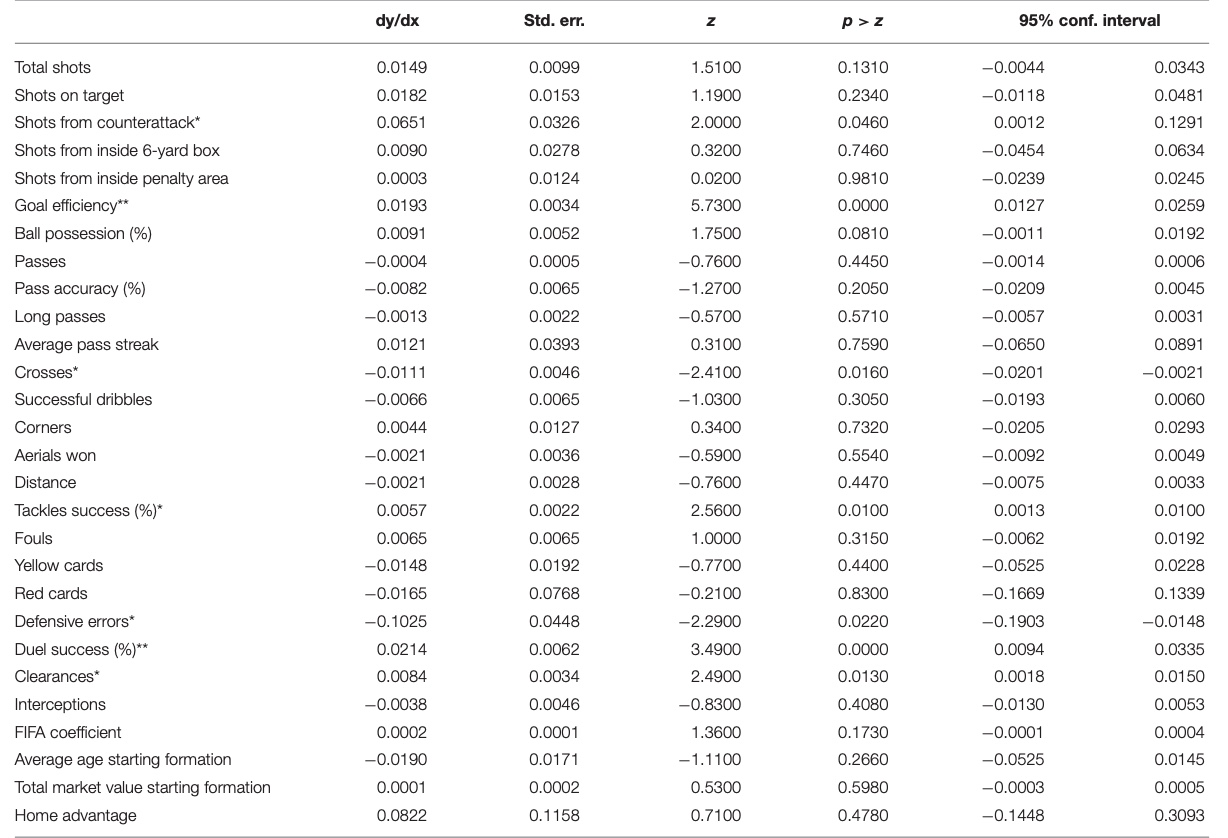
\includegraphics[width=1.0\textwidth]{Figs/Marginal Effects.jpeg} 
	\caption[Marginal Effects for the outcome "win"]{The marginal effects of each predictor variable on the outcome "win" }
\label{figure3}
\end{figure}



